%!TEX root = ED_Grafo.tex

\section{Travessia / Busca}
\begin{frame}[label=notas]
	\framesubtitle{Travessia/Percurso/Transversalização}

	Travessia: percorrer cada elemento ``uma'' vez.
	\\\vfill\pause
	Algoritmo Simples:\pause
	\begin{enumerate}
		\item Enquanto o conjunto $V$ de vértices não visitados não for vazio:
			\begin{enumerate}
				\item Retire um vértice $u$ de $V$.
				\item Processe o $u$.
				\item Insira $u$ no conjunto de vértices visitados $V'$
			\end{enumerate}
	\end{enumerate}
	% \begin{center}
 %  	\begin{minipage}{.8\textwidth}
%   	\begin{lstlisting}[morekeywords={travessia_em_grafos,estado_inicial,vazia,retira_um,objetivo,expande, e}]
% travessia_em_grafos(problema)
%     a_visitar:=  estado_inicial(problema)
%     nos_visitados:=  emptyset
%     enquanto(verdadeiro)
%         se(a_visitar= emptyset) retorna FALHA
%         folha:= retira_um(a_visitar)
%         se(folha = objetivo(problema)) retorna SUCESSO
%         nos_visitados += folha
%         para_cada(no pertence  expande(folha))
%             se(no nao_pertence a_visitar e no nao_pertence nos_visitados)
%                 a_visitar += no
% \end{lstlisting}
		% \end{minipage}
		% \end{center}
\end{frame}

\begin{frame}[label=notas]
	Busca:\pause\ \textbf{s. f.} 1. Ato de buscar. 2. Pesquisa.
	\\\vfill\pause
	Busca em uma estrutura de dados\alt<1-3>{?}{ é a aplicação de um algoritmo
	para encontrar um item específico em um conjunto de items (registros distintos,
	elementos de um domínio definido por uma função matemática, ou uma combinação
	de ambos).}\pause
	\\\vfill
	Algoritmo Simples:\pause
	\begin{enumerate}
		\item Enquanto o conjunto não for vazio:
			\begin{enumerate}
				\item \alert<6>{Escolha} um item do conjunto
				\item Se o item for o desejado, termine.
				\item Senão, retire-o do conjunto.
			\end{enumerate}
	\end{enumerate}
\end{frame}

\begin{frame}
	\framesubtitle{Busca em Profundidade}
	A estratégia é \alert{escolher o vértice mais profundo} para avaliação.
	\vfill
	\begin{center}
		\includegraphics<1 | handout:0>{dfs-progress01c}
		\includegraphics<2 | handout:0>{dfs-progress02c}
		\includegraphics<3 | handout:0>{dfs-progress03c}
		\includegraphics<4 | handout:0>{dfs-progress04c}
		\includegraphics<5 | handout:0>{dfs-progress05c}
		\includegraphics<6 | handout:0>{dfs-progress06c}
		\includegraphics<7 | handout:0>{dfs-progress07c}
		\includegraphics<8 | handout:0>{dfs-progress08c}
		\includegraphics<9 | handout:0>{dfs-progress09c}
		\includegraphics<10 | handout:0>{dfs-progress10c}
		\includegraphics<11 | handout:0>{dfs-progress11c}
		\includegraphics<12>{dfs-progress12c}
	\end{center}
\end{frame}

\begin{frame}
	\framesubtitle{Busca em Largura (em Extensão)}

	\begin{itemize}
		\item A estratégia é \alert{escolher o vértice mais raso} para avaliação.
		\item O algoritmo descobre todos os vértices a uma distância $k$ do vértice 
		origem antes de descobrir qualquer vértice a uma distância $k + 1$.
	\end{itemize}
	\vfill
	\begin{center}
		\includegraphics<1 | handout:0>{bfs-progress1c}
		\includegraphics<2 | handout:0>{bfs-progress2c}
		\includegraphics<3 | handout:0>{bfs-progress3c}
		\includegraphics<4 | handout:0>{bfs-progress4c}
	\end{center}
\end{frame}


% \begin{frame}[fragile,label=notas]
% 	\framesubtitle{Busca em Profundidade - Algoritmo}
	
% 	Enquanto a pilha não está vazia faça:
% 	\begin{enumerate}
% 		\item Seja  $v$  o vértice no topo da pilha e $A_V$ seus arcos.
% 		\item Se $A_V \neq \emptyset$, então retire uma aresta $(v,w)$ de $A_V$:
% 			\begin{itemize}
% 				\item Se $w$ não está marcado
% 				\begin{enumerate}[(i)]
% 					\item Então então marque $w$
% 					\item Coloque $w$ na lista de arcos visitados
% 				\end{enumerate} 
% 			\end{itemize} 
% 		\item Senão, retire $v$ do topo da pilha.
% 	\end{enumerate}
% \end{frame}


% \begin{frame}[label=notas]
% 	\framesubtitle{Busca em Largura (em Extensão) - Algoritmo}

% 	\begin{enumerate}
% 		\item Coloca o nó raiz na fila.
% 		\item Retira um nó do início da fila e o examina.
% 		\item Se o elemento procurado está nesse nó, interrompe a busca e retorna 
% 		o resultado.
% 		\item Senão, coloca todos os sucessores desse nó, ainda não 
% examinados, no final da lista. 
% 		\item Se a fila está vazia, cada nó no grafo já foi examinado
% 			\subitem{interrompe a busca e retorna ``não encontrado''.}
% 		\item Repete passo 2.
% 	\end{enumerate}
% \end{frame}

\begin{frame}
	\framesubtitle{Análise de Complexidade}
	
	\begin{itemize}[<+->]
		\item Estruturas de dados adequadas para cada busca?
		\item Complexidade temporal de ambos os algoritmos de busca é $O(|V|{\cdot}|A|)$.
		\vfill
		\item Complexidade espacial da busca em profundidade é $O(h)$, onde $h$ 
		é o comprimento do caminho mais longo no grafo.
		\item Complexidade espacial da busca em largura é $O(|V|{\cdot}|A|)$
	\end{itemize}
\end{frame}

\begin{frame}
	\framesubtitle{Busca Profundidade $x$ Largura}
	
	\begin{itemize}
		\item A busca em largura é completa apenas se nenhum vértice tem grau infinito\pause, a em profundidade se não houver um caminho de comprimento infinito.\vfill
		\item A busca em largura é ótima se o custo dos passos forem  idênticos.
		\pause\vfill
		\item A busca em profundidade é aplicada em vários algoritmos de ordenação 
		em grafos como:
		\begin{itemize}
	\item Ordenamento topológico.
	\item Encontrar componentes fortemente conectados.
		\end{itemize}
	\end{itemize}
\end{frame}

\newcommand{\sfrac}[2]{$^{#1}/_{#2}$}%
\newcommand{\canoaEsq}[2]{\sfrac{c#1}{#2}}%
\newcommand{\canoaDir}[2]{\sfrac{#1}{#2c}}%
\begin{frame}
	\framesubtitle{Exemplo de Aplicação: Missionários e Canibais}

	3 missionários e 3 canibais estão em um lado de um rio, e há uma canoa onde 
	cabem até 2 pessoas. Como levar todos ao outro lado do rio sem que, havendo 
	pelo menos um missionário na margem, não haja mais canibais que missionários 
	nela?
	\\\vfill\pause
	Supondo a representação: \LARGE \canoaEsq{MargemEsquerda}{MargemDireita}
\end{frame}

\newcommand{\ellipse}[2][blue]{%
	\draw[line width=1pt,#1] (#2) ellipse [x radius=1cm,y radius=.5cm];
}

\begin{frame}[label=notas]
	\framesubtitle{Exemplo: Missionários e Canibais}

	\Large
	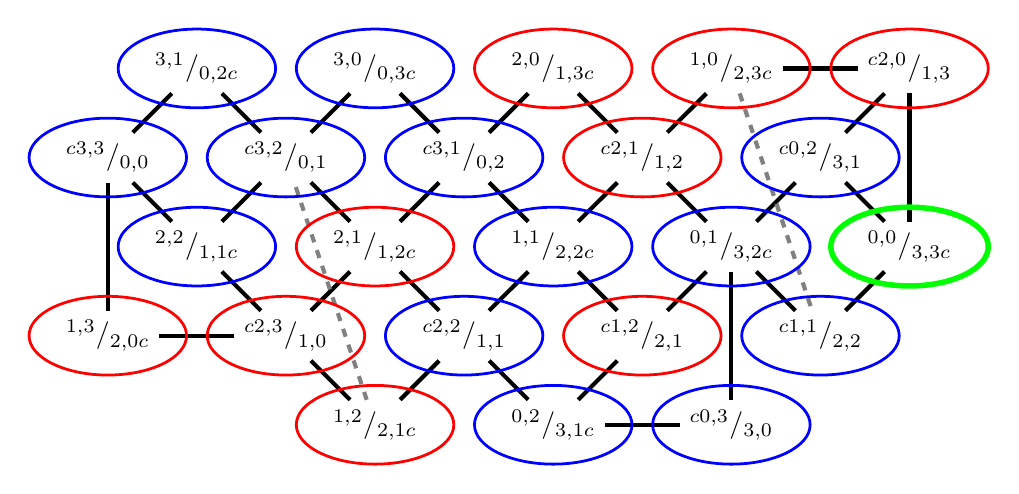
\begin{tikzpicture}[node distance=16mm]%[every node/.style={circle,draw},node distance=2cm]
		\node (c3300) {\canoaEsq{3,3}{0,0}};
		\pause
		%\node[above left of=c3300] (2310c) {\canoaDir{2,3}{1,0}} edge[line width=1.5pt] (c3300);
		%\node[below left of=c3300] (2301c) {\canoaDir{3,2}{0,1}} edge[line width=1.5pt] (c3300);
		\node[above right of=c3300] (3102c) {\canoaDir{3,1}{0,2}} edge[line width=1.5pt] (c3300);
		\node[below right of=c3300] (2211c) {\canoaDir{2,2}{1,1}} edge[line width=1.5pt] (c3300);
		\node[below left of=2211c] (1320c) {\canoaDir{1,3}{2,0}} edge[line width=1.5pt] (c3300);
		\pause
		\node[below right of=3102c] (c3201) {\canoaEsq{3,2}{0,1}} edge[line width=1.5pt] (3102c);
		\draw[line width=1.5pt] (c3201) -- (2211c);
		\node[below right of=2211c] (c2310) {\canoaEsq{2,3}{1,0}} edge[line width=1.5pt] (2211c);
		\draw[line width=1.5pt] (c2310) -- (1320c);
		\pause
		\node[above right of=c3201] (3003c) {\canoaDir{3,0}{0,3}} edge[line width=1.5pt] (c3201);
		\node[below right of=c3201] (2112c) {\canoaDir{2,1}{1,2}} edge[line width=1.5pt] (c3201);
		\draw[line width=1.5pt] (2112c) -- (c2310);
		\node[below right of=c2310] (1221c) {\canoaDir{1,2}{2,1}} edge[line width=1.5pt] (c2310);
		\draw[line width=1.5pt,dashed,gray] (1221c) -- (c3201);
		\pause
		\node[above right of=2112c] (c3102) {\canoaEsq{3,1}{0,2}} edge[line width=1.5pt] (2112c);
		\draw[line width=1.5pt] (3003c) -- (c3102);
		\node[above right of=1221c] (c2211) {\canoaEsq{2,2}{1,1}} edge[line width=1.5pt] (2112c);
		\draw[line width=1.5pt] (1221c) -- (c2211);
		\pause
		\node[above right of=c2211] (1122c) {\canoaDir{1,1}{2,2}} edge[line width=1.5pt] (c2211);
		\draw[line width=1.5pt] (1122c) -- (c3102);
		\node[above right of=c3102] (2013c) {\canoaDir{2,0}{1,3}} edge[line width=1.5pt] (c3102);
		\node[below right of=c2211] (0231c) {\canoaDir{0,2}{3,1}} edge[line width=1.5pt] (c2211);
		\pause
		\node[below right of=2013c] (c2112) {\canoaEsq{2,1}{1,2}} edge[line width=1.5pt] (2013c);
		\draw[line width=1.5pt] (c2112) -- (1122c);
		\node[below right of=1122c] (c1221) {\canoaEsq{1,2}{2,1}} edge[line width=1.5pt] (1122c);
		\draw[line width=1.5pt] (c1221) -- (0231c);
		\node[below right of=c1221] (c0330) {\canoaEsq{0,3}{3,0}} edge[line width=1.5pt] (0231c);
		\pause
		\node[above right of=c2112] (1023c) {\canoaDir{1,0}{2,3}} edge[line width=1.5pt] (c2112);
		\node[above right of=c1221] (0132c) {\canoaDir{0,1}{3,2}} edge[line width=1.5pt] (c1221);
		\draw[line width=1.5pt] (c2112) -- (0132c);
		\draw[line width=1.5pt] (c0330) -- (0132c);
		\pause
		\node[below right of=1023c] (c0231) {\canoaEsq{0,2}{3,1}} edge[line width=1.5pt] (0132c);
		\node[below right of=0132c] (c1122) {\canoaEsq{1,1}{2,2}} edge[line width=1.5pt] (0132c);
		\draw[line width=1.5pt,dashed,gray] (1023c) -- (c1122);
		\pause
		\node[below right of=c0231] (0033c) {\canoaDir{0,0}{3,3}} edge[line width=1.5pt] (c0231);
		\draw[line width=1.5pt] (0033c) -- (c1122);
		\node[above right of=c0231] (c2013) {\canoaEsq{2,0}{1,3}} edge[line width=1.5pt] (c0231);
		\draw[line width=1.5pt] (0033c) -- (c2013);
		\draw[line width=1.5pt] (1023c) -- (c2013);
		\pause
		\ellipse{c3300}
		\pause
		\ellipse{2211c}
		\ellipse{3102c}
		\ellipse[red]{1320c}
		\pause
		\ellipse{c3201}
		\ellipse[red]{c2310}
		\pause
		\ellipse{3003c}
		\ellipse[red]{2112c}
		\ellipse[red]{1221c}
		\pause
		\ellipse{c3102}
		\pause
		\ellipse{1122c}
		\ellipse[red]{2013c}
		\pause
		\ellipse[red]{c2112}
		\ellipse{c2211}
		\ellipse[red]{c1221}
		\pause
		\ellipse{0231c}
		\pause
		\ellipse{c0330}
		\pause
		\ellipse[red]{1023c}
		\ellipse[red]{c2013}
		\ellipse{0132c}
		\ellipse{c0231}
		\ellipse{c1122}
		\ellipse[green,line width=2pt]{0033c}
	\end{tikzpicture}
\end{frame}

\begin{frame}
	\framesubtitle{Exemplo: Missionários e Canibais}

	Supondo que só se explore nós que não violam as restrições e a representação $MCK$, onde:
	\begin{itemize}
		\item[M] número de missionários \emph{na margem errada}.
		\item[C] número de canibais \emph{na margem errada}.
		\item[K] número de canoas \emph{na margem errada}.
	\end{itemize}

	\vfill
	\begin{center}
		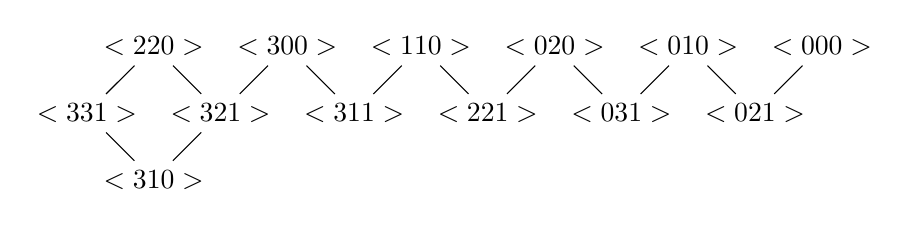
\begin{tikzpicture}[node distance=12mm]%
			\node (331){$<331>$};
			\pause
			\node[above right of=331] (220){$<220>$} edge (331);
			\node[below right of=331] (310){$<310>$} edge (331);
			\pause
			\node[below right of=220] (321){$<321>$} edge (220) edge (310);
			\pause
			\node[above right of=321] (300){$<300>$} edge (321);
			\node[below right of=300] (311){$<311>$} edge (300);
			\node[above right of=311] (110){$<110>$} edge (311);
			\node[below right of=110] (221){$<221>$} edge (110);
			\node[above right of=221] (020){$<020>$} edge (221);
			\node[below right of=020] (031){$<031>$} edge (020);
			\node[above right of=031] (010){$<010>$} edge (031);
			\node[below right of=010] (021){$<021>$} edge (010);
			\node[above right of=021] (000){$<000>$} edge (021);
		\end{tikzpicture}
	\end{center}
\end{frame}

\begin{frame}
	\framesubtitle{\url{http://www.youtube.com/watch?v=DINCL5cd_w0}}
	\begin{center}
		\href{run:vid/Pathfinding.mp4}{
\includegraphics[width=\textwidth]{dijkstra.png}}
	\end{center}
\end{frame}